% \label{chpt:results:evolutionary modelling} % for referencing this chapter elsewhere, use \ref{chpt:label}
% \lhead{\emph{Inferring mass loss rate from donor properties}} % This is for the header on each page - perhaps a shortened title

\label{chpt:Mass loss and Angular momentum loss in short period CVs} % for referencing this chapter elsewhere, use \ref{chpt:label}
\lhead{\emph{Mass loss and Angular momentum loss in short period CVs}} % This is for the header on each page - perhaps a shortened title

The structure of this chapter is as follows: first, I demonstrate that MESA is capable of reproducing the canonical CV donor tracks of \citet{knigge11}, and use MESA to evaluate the range of donor masses for which the method detailed in \S\ref{sect:modelling:evolutionary modelling} can be reasonably applied.
Then, I derive an empirical relationship for appropriate spot parameters as a function of donor mass, and use this to infer $\dot M_{\rm donor}$ and $\dot J$ for the well-characterised eclipse modelled CV sample.

The analysis of this section includes eclipse modelled data from several sources: the 15 systems contained in this thesis, the 15 CVs characterised by \citet{McAllister2019}, and the 14 CVs modelled by \citet{Savoury2011}. An additional 4 systems from \citet{mcallister2015,mcallister2017, mcallister2017b}; and \citet{copperwheat2010} were used, detailed in Table~\ref{appendix:table:supplementary systems}. A full catalogue of all these data is given in Appendix~\ref{appendix:eclipse modelled CV data tables}.
There is some overlap between the CVs contained in \citet{McAllister2019} and \citet{Savoury2011}, and where this is the case the more recent findings of \citet{McAllister2019} are preferred.


\section{Reproducing the canonical CV donor tracks}
\label{sect:results:reproducing K11 tracks}

MESA can closely reproduce the two \citet{knigge11} donor tracks. Recall from \S\ref{sect:introduction:the missing aml problem} that two such tracks are constructed, a `standard' track with only typical gravitational braking below the period gap, and an `optimal' track that amplifies gravitational braking by $2.47\times$.

Initial work to reproduce CV evolution is outlined in \citet{Paxton_2015}. A subsequent reproduction of the `optimal' track was undertaken by \citet{Pala2017a}, and I continue to refine their process.
By default, MESA shuts off magnetic braking when the donor becomes fully convective, a practice which I motivate in \S\ref{sect:introduction:the missing aml problem} to be spurious. Instead, MESA is altered to enforce a fixed magnetic braking cut-off at $0.2 M_\odot$, arbitrarily fixing the donor mass of the period gap in line with \citet{knigge11} (this is justified by observations - the mass of the period gap appears to be $0.20\pm0.02 M_\odot$ \citep{knigge11}).
In addition, \citet{Pala2017a} added a subroutine to MESA that allows for the amplification of gravitational braking below the period gap.
This subroutine uses the \lstinline{s% other_jdot_mb} MESA hook, and scales the calculated gravitational braking by a fixed constant below the period gap and applies it as magnetic braking. This was previously hard-coded, and I made minor changes to allow this scaling to be defined in the MESA configuration inlist.

This was used to reproduce the `optimal' track. Previous works have used entirely default MESA configuration for the donor physics, though I apply the configuration described in \S\ref{sect:modelling:MESA configs} to improve model accuracy. Beyond these settings, the model is also initialised with some additional binary configuration:
\begin{itemize}
    \item The two objects begin at an orbital period of 12 hours, with $M_{\rm donor} = 0.65 M_\odot$ and $M_{\rm wd} = 0.82$ to match the mean observed white dwarf mass. This period is chosen as the donor is not yet in contact with the Roche lobe but evolves to contact the Roche lobe relatively quickly.
    \item The donor mass at which the CV emerges from the period gap is dependent on spot parameters. The donor star has a fixed spot coverage $f_{\rm spot} = 0.10$ and contrast ratio of $x_{\rm spot} = 0$, chosen to approximately match the period at which the donor emerges from the period gap.
    \item The white dwarf is not allowed to retain any accreted material,
    \begin{itemize}
        \item \lstinline{mass_transfer_beta = 1.0}, \lstinline{limit_retention_by_mdot_edd = .false.}
    \end{itemize}
    \item The white dwarf is considered as a point mass, with no evolution over time,
    \begin{itemize}
        \item \lstinline{evolve_both_stars = .false.}
    \end{itemize}
\end{itemize}

These changes are enough to reproduce the \citet{knigge11} tracks to a reasonable degree; Figure~\ref{fig:results:MESA can reproduce the K11 tracks} shows the four model tracks in the short period regime.
Note that the small deviation at $\sim 0.13 M_\odot$ in the MESA models are due to MESA transitioning do a different equation of state, and is expected.
The small difference in gradient between the MESA models and the \citet{knigge11} models is due to the donor having a differing mass-radius relationship; this model does not use variable star spot physics as the donor mass falls.
With a more tailored donor configuration this could likely be improved without introducing the star spot physics at all -- specifically, the period minimum occurs at a significantly lower donor mass in the MESA models due to the differing equations of state and atmosphere tables used, but an exact reproduction of \citet{knigge11} is not the focus of this study and this agreement is considered acceptable.

\begin{figure}
    \centering
    \includegraphics[width=.9\textwidth]{figures/modelling/reproducing_K11_tracks_fspot0.100.pdf}
    \caption{Showing how well MESA can reproduce the canonical \citet{knigge11} donor tracks. {\bf Solid lines} are MESA tracks, and {\bf dotted lines} are the \citet{knigge11} tracks. {\bf Black} lines have only gravitational braking below the period gap, and {\bf red} lines gave gravitational braking at $2.47\times$ strength below the period gap.}
    \label{fig:results:MESA can reproduce the K11 tracks}
\end{figure}


\newpage
\section{For what range of masses can we extract mass loss rates?}
\label{sect:results:MESA massloss allowable mass range}

% This section evaluates the feasibility of using the radius of a star to extract present-day mass loss rates.
Note that the analysis of this section does not include any star spots, i.e. $f_{\rm spot} = 0$ for these models.

Recall from \S\ref{sect:introduction:period minimum and bouncers} the two timescales that govern the response of the donor to mass loss: $\tau_{\rm KH}$ and $\tau_{\dot M}$. These timescales are calculated by
\begin{align}
    \tau_{\rm KH} =& \frac{G M_{\rm donor}^2}{L_{\rm donor} R_{\rm donor}} \\[8pt]
    \tau_{\dot M} =& \frac{\dot M}{M_{\rm donor}}
\end{align}
If $\tau_{\rm KH} \ll \tau_{\dot M}$, the donor is able to maintain thermal equilibrium and is indistinguishable from a singleton star of the same mass.

If $\tau_{\rm KH} \gg \tau_{\dot M}$, the donor is not able to maintain equilibrium, and mass loss is fast and adiabatic.
The donor is inflated by mass loss, but since the stellar structure reacts relatively slowly, the adjustment of the structure towards equilibrium can be interrupted by changes in mass loss rate. This time lag between the star beginning to experience a specific mass loss rate, and the structure adjusting to reflect it makes the degree of inflation of the donor sensitive to the mass loss \textit{history} of the donor.
% The donor is inflated by mass loss, but because the stellar structure as a whole reacts relatively slowly, the effect of past mass loss is retained and the degree of inflation becomes sensitive to the mass loss \textit{history} of the donor.

Calculating the two timescales for CVs reveals that for much of their lives, $\tau_{\rm KH} \sim \tau_{\dot M}$ \citep{knigge11} - meaning that most CV donors are \textit{almost} able to maintain thermal equilibrium, but are still mildly affected by mass loss.
Under this almost-equilibrium regime, mass loss induces some degree of radius inflation in the donor, but because the star adjusts on timescales comparable to $\tau_{\dot M}$, the degree of inflation only depends on the present-day average $\dot M$. In this regime, we can discard the mass loss history of the donor, and use the radius inflation as a diagnostic for the baseline mass loss rate, averaged over $\tau_{\dot M} \sim 1$Gyr.
% This is also the justification for the CV tracks in \S\ref{sect:results:reproducing K11 tracks} to not include the star spot radius correction. As the donor decreases in mass, the necessary spot parameters to correct its radius will change (refer to \S\ref{sect:modelling:tuning star spots to observations}). However, the donor structure would only react to a change in spot parameters on the $\tau_{\rm KH}$ timescale, causing a CV donor model to effectively have the `wrong' spot parameters for its mass, due to the time lag between parameters changing and the donor radius responding to that change.


Whether a donor radius is sensitive to its $\dot M$ history is a function of $M_{\rm donor}$. As $M_{\rm donor}$ falls, $\tau_{\rm KH}$ begins to rise faster than $\tau_{\dot M}$. Figure~\ref{fig:results:how does tauKH and tauMdot vary with donor mass} shows this trend, produced by a MESA model of a CV using the configuration provided in \citet{Paxton_2015}.
The rise in $\tau_{\rm KH}$ relative to $\tau_{\dot M}$ becomes significant at $\sim 0.1 M_\odot$, around the mass the donor enters the adiabatic $\tau_{\rm KH} \gg \tau_{\dot M}$ period bouncer phase c.f.~\S\ref{sect:introduction:period minimum and bouncers}.
\begin{figure}
    \centering
    \includegraphics[width=\textwidth]{figures/modelling/tau_both_vs_donor_mass_AML000.pdf}
    \caption{Showing how the two timescales, $\tau_{\rm KH}$ and $\tau_{\dot M}$ vary with donor mass below the period gap in CV donors, as modelled by MESA \citep{Paxton_2015,Pala2017a}.}
    \label{fig:results:how does tauKH and tauMdot vary with donor mass}
\end{figure}

We can determine the range of donor masses for which $\tau_{\rm KH} \sim \tau_{\dot M}$ from MESA models.
First, a series of singleton models (this time using the MESA configuration given in \S\ref{sect:modelling:MESA configs}) were evaluated with varying amounts of fixed mass loss rates, uniformly spaced between $\log (\dot M, M_\odot \mathrm{yr}^{-1}) = -9.9 \rightarrow -10.8$.
Then, a series of MESA CV models were run with gravitational losses amplified by $x = 1 \rightarrow 6$, using the configuration and AML amplification in \S\ref{sect:results:reproducing K11 tracks}.
Finally, each model has its radius, $R$, and $\dot M$ extracted at $0.1 M_\odot$. Since the CV models have varying $\dot M$ and the singleton models do not, if $\dot M$ history does not affect radius inflation the radii between the two sets of models will match, and a disagreement indicates that history plays a significant role in radius inflation.
 Figure~\ref{fig:results:comparing radii at 0.1Msun} shows this, and little divergence between the two sets of radii is visible. Note that higher $\dot M$ show a small but increasing degree of divergence, as we might expect since higher $\dot M$ corresponds to lower $\tau_{\dot M}$.
\begin{figure}
    \centering
    \includegraphics[width=.8\textwidth]{figures/modelling/compare_0.1Msun_with_CV_track_K11_fig1.pdf}
    \caption{Showing the radius and mass loss extracted from MESA models at $0.1 M_\odot$. The {\bf black} line is a series of singleton models with constant mass loss, and the {\bf red} line is a series of CV models with gravitational AML amplified by $x = 1 \rightarrow 6$, with the lowest AML rate on the left. The {\bf blue dotted line} shows $\dot M$ for a CV with $2.47\times$ gravitational braking strength as predicted by a MESA CV model.}
    \label{fig:results:comparing radii at 0.1Msun}
\end{figure}

Now, by looking at what level of divergence historical changes in $\dot M$ induces at various donor masses, we can evaluate what mass range is acceptable.
By instead plotting the difference between the two sets of models, and repeating the same process for a range of masses, Figure~\ref{fig:results:comparing radii over a range of masses} is produced.
The upper limit on mass must be $0.2 M_\odot$, as this is the enforced mass of the period gap, and for a lower limit I impose an acceptable level of disagreement of $3\%$. It can be seen that the minimum acceptable mass is then $0.08 M_\odot$.
\begin{figure}
    \centering
    \includegraphics[width=\textwidth]{figures/modelling/compare_multiple_mass_with_CV_K11_fig1a.pdf}
    \caption{The inflation of CV model radii, $R_{CV}$ (whose $\dot M$ is time-dependent), over singleton model radii, $R_S$ (whose $\dot M$ is constant), from Figure~\ref{fig:results:comparing radii at 0.1Msun}, for a range of masses. The {\bf stars} on each line show the $\dot M$ and inflation for a model with gravitational braking at $2.47\times$ strength, mirroring the \citet{knigge11} optimal track. The {\bf red dashed line} shows the upper limit for acceptable disagreement, and the {\bf black dashed line} shows perfect agreement.}
    \label{fig:results:comparing radii over a range of masses}
\end{figure}


\newpage
\section{Tuning star spot parameters to observations}
\label{sect:modelling:tuning star spots to observations}

With star spots implemented in MESA in \S\ref{sect:modelling:starspots in MESA}, the Brown relation can now be reproduced.
For simplicity, $x_{\rm spot}$ is fixed at 0 and $f_{\rm spot}$ is varied.
Since radius increases monotonically with $f_{\rm spot}$, a binary chop is performed (see \S\ref{sect:modelling:binary chop methodology}), optimising for $\Delta R=R_{\rm MESA}-(1.045\times R_{\rm Brown})=0$ at a stellar age of 2~Gyrs for a range of masses. The 4.5\% radius increase is to compensate for the non-spherical Roche geometry of the donor, c.f. \citet{knigge11}.
The resulting M-$f_{\rm spot}$ relation is shown in Figure~\ref{fig:modelling:fspot mass relationship}.

Below masses of $\sim 0.12 M_\odot$, the required $f_{\rm spot}$ becomes slightly negative, i.e. default MESA models are larger than observations plus the $4.5\%$ non-spherical correction.
Since a negative coverage fraction is unphysical, negative values of $f_{\rm spot}$ are set equal to 0 and it should be emphasised that derived mass loss rates may become somewhat unreliable below this mass.
% Below $M_{\rm donor} = 0.121 M_\odot$ the Brown relation transitions to the \citet{baraffe2015} theoretical tracks, so model agreement is perhaps unsurprising here.
However, the clear trend in $f_{\rm spot}$ towards 0 prior to this, and the close proximity to $f_{\rm spot} = 0$ below $0.12 M_\odot$ suggests that the MESA radius calibration given here is still valid.
% The severity of this unreliability is not catastrophic, as the minimum value of $f_{\rm spot}$ is still reasonably close to 0.

There is significant scatter in the Brown mass-radius relation, that is not captured in these models. The inherent scatter in radius for the observations is $\sim 3\%$ between 0.1 and 0.2 $M_\odot$, which adds to the uncertainty in modelled radius inflation, and thus mass loss rate. Below $\sim 0.1 M_\odot$, the scatter is not able to be characterised.
Whilst this may skew an individual system, on average the inferred mass loss from model radius should be accurate. Therefore, this effect should not corrupt the $\dot M$ results with a large enough sample size.
Since the uncertainties I report here do not include the effects of the scatter in the Brown mass-radius relation, they are underestimates of the true uncertainty. However, due to the very poor constraints on the scatter, this effect is ignored until more information is available.

\begin{figure}
    \centering
    \includegraphics[width=\textwidth]{figures/modelling/fspot_relation_to_match_brown_plus_4.5.pdf}
    \caption{{\it Top}: The required $f_{\rm spot}$ that is applied to tune M dwarf MESA models to match the Brown relation, plus an added $4.5\%$ inflation due to non-spherical Roche geometry. {\it Bottom}: the residuals from the best fit value of $f_{\rm spot}$. The {\bf dotted lines} show the acceptable deviation from perfect agreement in order to terminate the binary chop, and the {\bf dashed line} shows the target inflation. Note that when finding the necessary value of $f_{\rm spot}$ to match the Brown relation $x_{\rm spot} \equiv 0$, and negative values of $f_{\rm spot}$ were allowed. However, in all subsequent modelling, negative $f_{\rm spot}$ were set to 0. {\bf Red squares} show evaluated MESA models.}
    \label{fig:modelling:fspot mass relationship}
\end{figure}



\section{Inferred mass and angular momentum loss rates from CV donors}
\label{sect:modelling:donor mass loss rates}

Overall, there are 33 systems with eclipse-modelled characterisations available with donors in the correct mass range of $0.08 M_\odot < M_{\rm donor} < 0.20 M_\odot$, catalogued in Table~\ref{table:results:mdot modelling}.

Table~\ref{table:results:Jdot results} shows the AML rates, $\dot J$, calculated using Equation~\ref{eqn:modelling:Jdot from Mdot} for the systems for which $\dot M$ could be calculated from donor properties. Also shown is the AML expected from gravitational losses alone for that system, and the ratio between the observed and expected values.

Two systems appear to have less AML than is predicted by gravitational losses: ASASSN-17fo (from Chapter~\ref{chpt:characterisation of 12 new CVs}) and SDSS J0903 \citep{Savoury2011}, and an erroneous eclipse model result can be eliminated in each case.
ASASSN-17fo is confidently eclipse modelled, with distinct, well modelled eclipse features and a good white dwarf flux fit, so is unlikely to be unreliable. SDSS J0903 also has a confident eclipse model fit. Whilst the bright spot features of this system are less distinct, the fitting results are satisfactory.
However, the inferred $\dot M$ is contingent on a chain of assumptions all holding true; the eclipse modelling must be robust, the MESA configuration must be accurate \textit{for the specific donor being considered}, and the equilibrium radius of the donor in question must be well-described by the Brown relation. A failure in any of these steps will produce incorrect values of $\dot M$ and $\dot J$, and the consequences of the breakdown of these assumptions is discussed in \S\ref{sect:massloss and AML:systematic bias}.

Aside from these two cases the inferred $\dot M$ are generally physically reasonable, suggesting that the general data set is acceptable for preliminary analysis. In the interests of honest analysis, the two sub-gravitational loss CVs are still included in the following examination of the data.


\begin{table*}
    \centering
    \caption{The inferred $\dot M$ for eclipse-modelled CVs. For the Source column, `W22' are from Chapter~\ref{chpt:characterisation of 12 new CVs}, `M19' are systems modelled by \citet{McAllister2019}, `M17b' is from \citet{mcallister2017b}, `S11' are from \citet{Savoury2011}}
    \label{table:results:mdot modelling}
    \begin{tabular}{llccc}
        \hline \\
        {\bf System Name:} & \textbf{Source} & \textbf{$M_{\rm donor}, M_\odot$}  & \textbf{$R_{\rm donor}, R_\odot$}  & \textbf{$\log_{10}(\dot M,\ M_\odot / {\rm yr})$} \\
        \hline \hline \\
        ASASSN-14hq         &  W22      & $0.097 \pm 0.002$ & $0.157 \pm 0.001$ & $ -9.897 \pm 0.008$ \\
        ASASSN-15pb         &  W22      & $0.148 \pm 0.008$ & $0.209 \pm 0.003$ & $ -9.997 \pm 0.164$ \\
        ASASSN-17fo         &  W22      & $0.109 \pm 0.001$ & $0.144 \pm 0.001$ & $-10.859 \pm 0.137$ \\
        AY For              &  W22      & $0.106 \pm 0.005$ & $0.162 \pm 0.002$ & $ -9.918 \pm 0.024$ \\
        CSS090419           &  W22      & $0.087 \pm 0.016$ & $0.152 \pm 0.006$ & $ -9.859 \pm 0.003$ \\
        CSS090622           &  W22      & $0.105 \pm 0.009$ & $0.155 \pm 0.004$ & $-10.046 \pm 0.074$ \\
        MASTER OT J0014     &  W22      & $0.123 \pm 0.006$ & $0.165 \pm 0.002$ & $-10.279 \pm 0.328$ \\
        OGLE82              &  W22      & $0.132 \pm 0.003$ & $0.170 \pm 0.001$ & $-11.686 \pm 1.078$ \\
        SDSS J0748          &  W22      & $0.085 \pm 0.010$ & $0.128 \pm 0.005$ & $-10.438 \pm 0.152$ \\
        SDSS J1524          &  W22      & $0.097 \pm 0.003$ & $0.144 \pm 0.001$ & $-10.210 \pm 0.030$ \\
        CSS080623           &  M19      & $0.081 \pm 0.005$ & $0.128 \pm 0.002$ & $-10.343 \pm 0.041$ \\
        CSS110113           &  M19      & $0.105 \pm 0.007$ & $0.149 \pm 0.003$ & $-10.272 \pm 0.129$ \\
        OY Car              &  M19      & $0.093 \pm 0.004$ & $0.139 \pm 0.001$ & $-10.278 \pm 0.046$ \\
        SDSS J0901          &  M19      & $0.138 \pm 0.007$ & $0.182 \pm 0.003$ & $-10.547 \pm 0.368$ \\
        SDSS J1152          &  M19      & $0.094 \pm 0.016$ & $0.147 \pm 0.006$ & $-10.062 \pm 0.156$ \\
        SSS100615           &  M19      & $0.083 \pm 0.005$ & $0.128 \pm 0.002$ & $-10.384 \pm 0.038$ \\
        ASASSN-14ag         &  M17b     & $0.093 \pm 0.010$ & $0.135 \pm 0.007$ & $-10.416 \pm 0.211$ \\
        CTCV J2354-4700     &  S11      & $0.101 \pm 0.003$ & $0.146 \pm 0.001$ & $-10.245 \pm 0.030$ \\
        % SDSS J1152          &  S11      & $0.087 \pm 0.006$ & $0.142 \pm 0.003$ & $-10.068 \pm 0.025$ \\
        OU Vir              &  S11      & $0.116 \pm 0.002$ & $0.163 \pm 0.001$ & $-10.067 \pm 0.026$ \\
        XZ Eri              &  S11      & $0.091 \pm 0.004$ & $0.135 \pm 0.001$ & $-10.352 \pm 0.054$ \\
        SDSS J0903          &  S11      & $0.099 \pm 0.004$ & $0.136 \pm 0.002$ & $-10.677 \pm 0.155$ \\
        SDSS J1227          &  S11      & $0.089 \pm 0.002$ & $0.137 \pm 0.001$ & $-10.243 \pm 0.017$ \\
        SDSS J1502          &  S11      & $0.078 \pm 0.001$ & $0.124 \pm 0.001$ & $-10.377 \pm 0.008$ \\
        ASASSN-14kb         &  W22      & $0.134 \pm 0.003$ & $0.164 \pm 0.001$ & -                   \\
        CTCV 1300-3052      &  M19      & $0.166 \pm 0.006$ & $0.211 \pm 0.002$ & -                   \\
        DV UMa              &  M19      & $0.187 \pm 0.012$ & $0.215 \pm 0.005$ & -                   \\
        IY UMa              &  M19      & $0.141 \pm 0.007$ & $0.177 \pm 0.002$ & -                   \\
        SSS130413           &  M19      & $0.140 \pm 0.012$ & $0.163 \pm 0.004$ & -                   \\
        V713 Cep            &  M19      & $0.176 \pm 0.018$ & $0.208 \pm 0.005$ & -                   \\
        Z Cha               &  M19      & $0.152 \pm 0.005$ & $0.182 \pm 0.002$ & -                   \\
        CTCV J1300-3052     &  S11      & $0.177 \pm 0.021$ & $0.215 \pm 0.008$ & -                   \\
        DV UMa              &  S11      & $0.196 \pm 0.005$ & $0.218 \pm 0.001$ & -                   \\
        % CSS090102           &  W22      & $0.059 \pm 0.003$ & $0.119 \pm 0.002$ & $-10.255 \pm 0.024$ \\
        % ASASSN-16kr         &  W20      & $0.042 \pm 0.003$ & $0.106 \pm 0.002$ & $-10.672 \pm 0.274$ \\
        % SSSJ1502-3505       &  W20      & $0.042 \pm 0.003$ & $0.106 \pm 0.003$ & $-10.648 \pm 0.206$ \\
        % SDSS 1501           &  M19      & $0.061 \pm 0.004$ & $0.113 \pm 0.002$ & $-10.456 \pm 0.034$ \\
        % SDSS J1057+2759     &  M17a     & $0.044 \pm 0.002$ & $0.109 \pm 0.001$ & $-10.514 \pm 0.102$ \\
        % PHL 1445            &  M15      & $0.064 \pm 0.005$ & $0.109 \pm 0.004$ & $-10.660 \pm 0.101$ \\
        % SDSS 1035           &  S11      & $0.048 \pm 0.001$ & $0.105 \pm 0.001$ & $-10.742 \pm 0.011$ \\
        % SDSS J1501          &  S11      & $0.077 \pm 0.010$ & $0.122 \pm 0.005$ & $-10.429 \pm 0.066$ \\
        % ASASSN-17jf         &  W20      & $0.060 \pm 0.008$ & $0.112 \pm 0.004$ & -                   \\
        % GY Cnc              &  M19      & $0.394 \pm 0.022$ & $0.446 \pm 0.009$ & -                   \\
        % SDSS 1006           &  M19      & $0.370 \pm 0.060$ & $0.457 \pm 0.026$ & -                   \\
        % SDSS 1702           &  S11      & $0.223 \pm 0.010$ & $0.252 \pm 0.004$ & -                   \\
        % SDSS 1507           &  S11      & $0.058 \pm 0.002$ & $0.097 \pm 0.001$ & -                   \\
        % SDSS 1433           &  S11      & $0.057 \pm 0.001$ & $0.107 \pm 0.001$ & -                   \\
        % IP Peg              &  C10      & $0.550 \pm 0.020$ & $0.466 \pm 0.006$ & -                   \\
        \hline
    \end{tabular}
\end{table*}

\begin{table*}
    \centering
    \caption{The inferred AML rates for the CVs in this sample. $\dot J_{\rm total}$ is calculated from the inferred $\dot M$, and $\dot J_{\rm GR}$ is the calculated gravitational AML rate. Sources are keyed the same as Table~\ref{table:results:mdot modelling}.}
    \label{table:results:Jdot results}
    \begin{tabular}{llccc}
        \hline
        {\bf System Name:} & \textbf{Source}  & \textbf{$\log(\dot J_{\rm total}, J)$} & \textbf{$\log(\dot J_{\rm GR}, J)$} & \textbf{$\dot J_{\rm total} / \dot J_{\rm GR}$} \\
        \hline \hline
        ASASSN-14hq     &  W22      & $27.157 \pm 0.009$    & $26.681 \pm 0.007$    & $2.996 \pm 0.081$ \\
        ASASSN-15pb     &  W22      & $27.091 \pm 0.162$    & $26.796 \pm 0.013$    & $2.115 \pm 0.818$ \\
        ASASSN-17fo     &  W22      & $26.240 \pm 0.137$    & $26.711 \pm 0.004$    & $0.355 \pm 0.114$ \\
        AY For          &  W22      & $27.184 \pm 0.026$    & $26.705 \pm 0.015$    & $3.021 \pm 0.204$ \\
        CSS090419       &  W22      & $27.158 \pm 0.039$    & $26.634 \pm 0.058$    & $3.381 \pm 0.548$ \\
        CSS090622       &  W22      & $26.994 \pm 0.078$    & $26.699 \pm 0.028$    & $2.011 \pm 0.388$ \\
        MASTER OT J0014 &  W22      & $26.842 \pm 0.325$    & $26.745 \pm 0.014$    & $1.661 \pm 1.488$ \\
        OGLE82          &  W22      & $25.428 \pm 1.083$    & $26.767 \pm 0.009$    & $0.980 \pm 8.280$ \\
        SDSS J0748      &  W22      & $26.645 \pm 0.156$    & $26.629 \pm 0.053$    & $1.116 \pm 0.442$ \\
        SDSS J1524      &  W22      & $27.027 \pm 0.031$    & $26.723 \pm 0.043$    & $2.027 \pm 0.234$ \\
        CSS080623       &  M19      & $26.705 \pm 0.042$    & $26.615 \pm 0.026$    & $1.238 \pm 0.141$ \\
        CSS110113       &  M19      & $26.895 \pm 0.128$    & $26.701 \pm 0.019$    & $1.633 \pm 0.502$ \\
        OY Car          &  M19      & $26.844 \pm 0.046$    & $26.666 \pm 0.014$    & $1.517 \pm 0.168$ \\
        SDSS J0901      &  M19      & $26.536 \pm 0.368$    & $26.780 \pm 0.014$    & $0.815 \pm 0.870$ \\
        SDSS J1152      &  M19      & $26.954 \pm 0.157$    & $26.656 \pm 0.073$    & $2.149 \pm 0.894$ \\
        SSS100615       &  M19      & $26.730 \pm 0.039$    & $26.625 \pm 0.024$    & $1.282 \pm 0.138$ \\
        ASASSN-14ag     &  M17b     & $26.587 \pm 0.215$    & $26.657 \pm 0.056$    & $0.968 \pm 0.526$ \\
        CTCV J2354-4700 &  S11      & $26.899 \pm 0.032$    & $26.691 \pm 0.008$    & $1.616 \pm 0.122$ \\
        % SDSS J1152      &  S11      & $26.917 \pm 0.030$    & $26.642 \pm 0.026$    & $1.893 \pm 0.172$ \\
        OU Vir          &  S11      & $26.992 \pm 0.027$    & $26.729 \pm 0.005$    & $1.837 \pm 0.117$ \\
        XZ Eri          &  S11      & $26.721 \pm 0.054$    & $26.659 \pm 0.015$    & $1.164 \pm 0.151$ \\
        SDSS J0903      &  S11      & $26.427 \pm 0.154$    & $26.685 \pm 0.012$    & $0.587 \pm 0.217$ \\
        SDSS J1227      &  S11      & $26.848 \pm 0.018$    & $26.652 \pm 0.010$    & $1.572 \pm 0.075$ \\
        SDSS J1502      &  S11      & $26.669 \pm 0.009$    & $26.602 \pm 0.005$    & $1.169 \pm 0.026$ \\
        % CSS090102       &  W22      & $26.768 \pm 0.027$    & $26.422 \pm 0.046$    & $2.235 \pm 0.273$ \\
        % ASASSN-16kr     &  W20      & $26.490 \pm 0.276$    & $26.059 \pm 0.093$    & $3.375 \pm 2.522$ \\
        % SSSJ1502-3505   &  W20      & $26.446 \pm 0.209$    & $26.070 \pm 0.103$    & $2.737 \pm 1.564$ \\
        % SDSS 1501       &  M19      & $26.600 \pm 0.035$    & $26.448 \pm 0.052$    & $1.435 \pm 0.210$ \\
        % SDSS J1057      &  M17a     & $26.598 \pm 0.103$    & $26.109 \pm 0.056$    & $3.203 \pm 0.874$ \\
        % PHL 1445        &  M15      & $26.386 \pm 0.101$    & $26.482 \pm 0.057$    & $0.830 \pm 0.226$ \\
        % SDSS 1035       &  S11      & $26.365 \pm 0.011$    & $26.212 \pm 0.029$    & $1.426 \pm 0.101$ \\
        % SDSS 1501       &  S11      & $26.639 \pm 0.067$    & $26.581 \pm 0.072$    & $1.169 \pm 0.271$ \\
        % ASASSN-14kb     &  W22      & $   NaN \pm   NaN$    & $26.772 \pm 0.009$    & $  NaN \pm   NaN$ \\
        % ASASSN-17jf     &  W20      & $   NaN \pm   NaN$    & $26.416 \pm 0.127$    & $  NaN \pm   NaN$ \\
        % CTCV 1300-3052  &  M19      & $   NaN \pm   NaN$    & $26.821 \pm 0.008$    & $  NaN \pm   NaN$ \\
        % DV UMa          &  M19      & $   NaN \pm   NaN$    & $27.036 \pm 0.463$    & $  NaN \pm   NaN$ \\
        % GY Cnc          &  M19      & $   NaN \pm   NaN$    & $28.717 \pm 0.053$    & $  NaN \pm   NaN$ \\
        % IY UMa          &  M19      & $   NaN \pm   NaN$    & $26.785 \pm 0.013$    & $  NaN \pm   NaN$ \\
        % SDSS 1006       &  M19      & $   NaN \pm   NaN$    & $28.647 \pm 0.179$    & $  NaN \pm   NaN$ \\
        % SSS130413       &  M19      & $   NaN \pm   NaN$    & $26.781 \pm 0.023$    & $  NaN \pm   NaN$ \\
        % V713 Cep        &  M19      & $   NaN \pm   NaN$    & $26.953 \pm 0.388$    & $  NaN \pm   NaN$ \\
        % Z Cha           &  M19      & $   NaN \pm   NaN$    & $26.803 \pm 0.007$    & $  NaN \pm   NaN$ \\
        % CTCV J1300-3052 &  S11      & $   NaN \pm   NaN$    & $27.023 \pm 0.476$    & $  NaN \pm   NaN$ \\
        % DV UMa          &  S11      & $   NaN \pm   NaN$    & $27.142 \pm 0.530$    & $  NaN \pm   NaN$ \\
        % SDSS 1702       &  S11      & $   NaN \pm   NaN$    & $28.218 \pm 0.140$    & $  NaN \pm   NaN$ \\
        % SDSS 1507       &  S11      & $   NaN \pm   NaN$    & $26.402 \pm 0.030$    & $  NaN \pm   NaN$ \\
        % SDSS 1433       &  S11      & $   NaN \pm   NaN$    & $26.399 \pm 0.011$    & $  NaN \pm   NaN$ \\
        % IP Peg          &  C10      & $   NaN \pm   NaN$    & $29.061 \pm 0.034$    & $  NaN \pm   NaN$ \\
        \hline
    \end{tabular}
\end{table*}


\subsection{Systematic issues with mass loss estimation}
\label{sect:massloss and AML:systematic bias}

It is critical to treat these mass loss rates with caution.
The sample as given here is subject to systematic bias as a result of the sparse nature of the data used to calibrate the Brown relation, and the validity of $\dot M$ and $\dot J$ is sensitive to the validity of the MESA configuration for the donor model.
Whilst the majority of CV donors are probably well-described by my MESA configuration, we cannot assume that \textit{all} donors will be; the configuration could easily be invalidated by, for example, the presence of a more evolved donor, or one with a substantially different metallicity from typical M dwarfs.
This would alter the mass-radius exponent of the donor ($\zeta$ in Equation~\ref{eqn:modelling:Jdot from Mdot}) and corrupt the inferred $\dot J$.

Beyond a potentially incorrect MESA configuration, there is a more serious problem with the unknown scatter in the Brown relation.
Consider a star which lies below the Brown relation, i.e. one with a smaller zero-$\dot M$ radius than its mass suggests. If this star begins to experience mass loss, and we measure its radius to be inflated beyond the Brown relation (after factoring for Roche geometry), the corresponding mass loss rate we would find will be \textit{lower} than reality, as some amount of the star's inflation -- the amount required to inflate it to agree with the Brown relation -- is ignored.
This is illustrated in Figure~\ref{fig:massloss and AML:brown scatter causes bias}.
This will also cause some stars to fail to have $\dot M$ inferred. If the zero-$\dot M$ radius is small enough, it becomes likely that the amount of inflation induced by mass loss is not sufficient to bring the star up to the radius assumed by the Brown relation. Such a donor would not be possible to reproduce using this methodology, and 9 such donors (approximately a quarter of the sample) are seen in Table~\ref{table:results:mdot modelling}.
\begin{figure}
    \centering
    \includegraphics[width=.7\textwidth]{figures/results/brown_scatter_causes_bias.png}
    \caption{Illustrating how scatter about the Brown relation can corrupt inferred $\dot M$ rates. The upper solid black line shows the observed radius of a donor, and the lower three lines show possible zero $\dot M$ radii. The dotted black line shows the radius predicted by the Brown relation. The arrows show the amount of inflation induced by $\dot M$, with longer arrows requiring more $\dot M$. The black arrow shows the reported value, but assumes the donor would exactly agree with the Brown relation. If the zero-$\dot M$ radius of a donor corresponds to star A (blue line), some extra $\dot M$ will be incorrectly attributed to the system (shown as the dotted section). If the zero-$\dot M$ radius of the donor corresponds to star B (red line), some amount of $\dot M$ will be ignored (again shown as the dotted section).}
    \label{fig:massloss and AML:brown scatter causes bias}
\end{figure}

The combination of these two effects makes our dataset as a whole systematically over-estimate $\dot M$. This is because systems with donors that scatter below the Brown relation are preferentially removed from the sample -- they are more likely to have inflations that lie below the baseline radius (i.e. they lie below the dotted black line in Figure~\ref{fig:massloss and AML:brown scatter causes bias}), and are systems which would have had their $\dot M$ under-estimated.
Donors which scatter above the Brown relation are not removed in this way, so over-estimated $\dot M$ become over-represented in the sample.
Some portion of systems are, for the same reasons, reported with abnormally low $\dot M$ -- i.e. ASASSN-17fo and SDSS J0903 -- as their donors scatter below the Brown relation, but not by enough as to remove them from the sample.
Finally, since our reported $\dot M$ do not consider the intrinsic scatter in the M dwarf population, the uncertainties in $\dot M$ reported are likely to be significantly under-estimated.

Although this bias presents a problem for quantitative analysis, the general trends that these data show can still be considered generally correct, with the caveat that these are preliminary results. A larger sample of M dwarf masses and radii in the $M < 0.2 M_\odot$ range to give a better mass-radius relationship is highly desirable, and is likely to be provided in the near future with the release of Gaia DR3.
With a proper characterisation of the intrinsic population scatter, it will be possible to marginalise over the scatter to remove the over-estimation of $\dot M$, more faithfully report uncertainties, and perform more rigorous quantitative analysis of the data.



\section{Mass loss from white dwarf properties}
\label{sect:modelling:white dwarf mass loss rates}

% The characterised CVs also have the white dwarf temperature constrained to within $\sim 2000 \rm K$, allowing the short-term mass loss rate to also be inferred as suggested in \S\ref{sect:modelling:mdot from wd temperature}.
% Note that, despite the large uncertainty in $T_{\rm eff}$, the errors are smaller than those obtained with the donor properties.
% Figure~\todo{Get this figure} compares the $\dot M$ found by each technique, plotted as a function of donor mass.


The white dwarf temperature also reveals information on the mass transfer rate, and the following summary is described more quantitatively by \citet{townsley2009}.
In brief, as accreted material strikes the surface of the white dwarf its kinetic energy is converted to thermal energy, heating the white dwarf surface.
The degree of this heating is related to the rate at which material falls to the surface -- if more material falls in, more heating is induced.
Since, in general, we can assume that the rate material falls onto the white dwarf is roughly equal to the rate at which material enters the accretion disc from the donor, the white dwarf $T_{\rm eff}$ becomes a proxy diagnostic of the donor $\dot M$.
Simulations demonstrate that even through successive Nova eruptions, the core temperature of the white dwarf is stable over timescales of $\sim 10^8$ years \citep{epelstain2007}, so if the accretion rate falls, the white dwarf $T_{\rm eff}$ is able to cool to the appropriate, lower temperature and remain accurate to the present-day accretion rate.

The white dwarf temperature approach holds a major advantage over using the donor properties: measurements of white dwarf temperatures are easier to gather in large sample sizes.
However, the white dwarf temperature is capable of responding to changes in $\dot M$ on $\tau_{\rm Twd} \sim 10^3 - 10^5\ {\rm yrs}$ \citep{townsley2009}, as opposed to the $\rm \sim~Gyr$ timescales of the donor-based method described in \S\ref{sect:modelling:donor mass loss rates}, thus the $\dot M$ inferred from the white dwarf is averaged over $\tau_{\rm Twd}$ and only provides a short-term snapshot of the $\dot M$ and is susceptible to corruption from outbursts.
% In addition, the method assumes that the white dwarf is not a helium-core white dwarf, which is not always the case in the CV population and introduces significant unmodelled scatter to the results.

The short-term average mass loss rate, $\langle\dot M\rangle$, is ultimately a function only of white dwarf mass, and temperature, given in Equation~\ref{eqn:modelling:Mdot from wd temperature}.
\begin{equation}
    \label{eqn:modelling:Mdot from wd temperature}
    T_{\rm eff} = 1.7 \times 10^4 {\rm K} \bigg( \frac{\langle\dot M\rangle}{10^{-10} M_\odot {\rm yr}^{-1}} \bigg)^{1/4} \bigg( \frac{M_{\rm wd}}{0.9 M_\odot} \bigg)
\end{equation}

Recently, \citet{Pala2021} used spectroscopically estimated $T_{\rm eff}$ and $M_{\rm wd}$ to infer the $\dot M$ of 65 CVs. %, the result of which is reproduced in Figure~\ref{fig:modelling:pala2022 fig13}.
One finding from this analysis was an inverse correlation between $M_{\rm wd}$ and $\dot M$, contrary to the prediction of gravitational wave braking that lower mass systems should have lower AML rates driving lower $\dot M$.
As the eclipse modelling of CVs also produces a measure of $T_{\rm eff}$, the systems analysed for this thesis can be processed with {\it both} techniques, and have their results compared. Table~\ref{table:results:Mdot from white dwarf parameters} shows the resulting $\dot M$ from the white dwarf parameters.
% \begin{figure}
%     \centering
%     \includegraphics[width=\textwidth]{figures/modelling/pala_2022_fig13.png}
%     \caption{Reproduced from \citet{Pala2021}, Figure~13. The subset of modelled systems, with $P < 3{\rm hr}$ are shown. {\bf Circles} and {\bf stars} are pre- and post-period bounce systems derived by \citet{Pala2021}, and {\bf diamonds} and {\bf pentagons} are pre- and post-period bounce systems taken from the literature. {\it Left}: The $T_{\rm eff}$ is plotted against $M_{\rm wd}$, and no correlation can be seen. {\it Right}: $\log \langle \dot M \rangle$ is plotted against $M_{\rm wd}$, though now the data are correlated along the white dwarf mass-radius relationship outlined by \citet{Pala2021}, $M_{\rm wd} \propto R_{\rm wd}^{2}$, shown by the {\bf black line}.}
%     \label{fig:modelling:pala2022 fig13}
% \end{figure}


\begin{table}
    \centering
    \caption{The $\dot M$ found using the white dwarf properties for each system with a $\dot M$ measurement from donor properties. Sources are keyed the same as Table~\ref{table:results:mdot modelling}}
    \label{table:results:Mdot from white dwarf parameters}
    \begin{tabular}{llccc}
        \hline
        \textbf{Name} & \textbf{Source} & \textbf{$M_{\rm wd}, M_\odot$} & \textbf{$T_{\rm eff}$, K} & \textbf{$\log (\dot M, M_\odot {\rm yr}^{-1})$} \\
        \hline \hline \\
        ASASSN-14hq      &  W22  & $0.67 \pm 0.01$ & $14800\pm   800$ & $ -9.93 \pm 0.02$ \\
        ASASSN-14kb      &  W22  & $0.74 \pm 0.02$ & $17700\pm  1000$ & $ -9.90 \pm 0.03$ \\
        ASASSN-15pb      &  W22  & $0.72 \pm 0.03$ & $19200\pm  1600$ & $ -9.85 \pm 0.04$ \\
        ASASSN-17fo      &  W22  & $0.85 \pm 0.01$ & $14800\pm   600$ & $-10.03 \pm 0.02$ \\
        AY For           &  W22  & $0.78 \pm 0.02$ & $18200\pm   500$ & $ -9.91 \pm 0.02$ \\
        CSS090102        &  W22  & $0.62 \pm 0.03$ & $14800\pm  1200$ & $ -9.90 \pm 0.04$ \\
        CSS090419        &  W22  & $0.59 \pm 0.08$ & $18200\pm  9000$ & $ -9.79 \pm 0.28$ \\
        CSS090622        &  W22  & $0.67 \pm 0.06$ & $ 9800\pm  1500$ & $-10.11 \pm 0.08$ \\
        MAS0014          &  W22  & $0.86 \pm 0.03$ & $17300\pm  1000$ & $ -9.97 \pm 0.03$ \\
        OGLE82           &  W22  & $0.84 \pm 0.02$ & $18000\pm  4400$ & $ -9.95 \pm 0.12$ \\
        SDSS J0748       &  W22  & $0.80 \pm 0.05$ & $28400\pm  3300$ & $ -9.73 \pm 0.06$ \\
        SDSS J1524       &  W22  & $0.99 \pm 0.01$ & $12500\pm   900$ & $-10.17 \pm 0.03$ \\
        ASASSN-16kr      &  W20  & $0.95 \pm 0.02$ & $11500\pm   300$ & $-10.19 \pm 0.01$ \\
        ASASSN-17jf      &  W20  & $0.70 \pm 0.03$ & $12020\pm   850$ & $-10.03 \pm 0.04$ \\
        SSSJ1502-3505    &  W20  & $0.76 \pm 0.02$ & $22800\pm  1500$ & $ -9.80 \pm 0.03$ \\
        CSS080623        &  M19  & $0.71 \pm 0.02$ & $15500\pm  1700$ & $ -9.94 \pm 0.05$ \\
        CSS110113        &  M19  & $1.00 \pm 0.05$ & $14500\pm  2200$ & $-10.11 \pm 0.07$ \\
        CTCV 1300-3052   &  M19  & $0.72 \pm 0.02$ & $11000\pm  1000$ & $-10.09 \pm 0.04$ \\
        DV UMa           &  M19  & $1.09 \pm 0.03$ & $17400\pm  1900$ & $-10.07 \pm 0.05$ \\
        GY Cnc           &  M19  & $0.88 \pm 0.02$ & $25900\pm  2300$ & $ -9.81 \pm 0.04$ \\
        IY UMa           &  M19  & $0.96 \pm 0.01$ & $18000\pm  1000$ & $-10.00 \pm 0.02$ \\
        OY Car           &  M19  & $0.88 \pm 0.02$ & $18600\pm  2800$ & $ -9.95 \pm 0.07$ \\
        SDSS J0901       &  M19  & $0.75 \pm 0.02$ & $14900\pm  2000$ & $ -9.98 \pm 0.06$ \\
        SDSS J1006       &  M19  & $0.82 \pm 0.11$ & $16500\pm  2000$ & $ -9.97 \pm 0.08$ \\
        SDSS J1152       &  M19  & $0.62 \pm 0.04$ & $15900\pm  2000$ & $ -9.87 \pm 0.06$ \\
        SDSS J1501       &  M19  & $0.72 \pm 0.02$ & $14900\pm  1000$ & $ -9.96 \pm 0.03$ \\
        SSS100615        &  M19  & $0.88 \pm 0.03$ & $13600\pm  1500$ & $-10.09 \pm 0.05$ \\
        SSS130413        &  M19  & $0.84 \pm 0.03$ & $24000\pm  3000$ & $ -9.82 \pm 0.06$ \\
        V713 Cep         &  M19  & $0.70 \pm 0.02$ & $17000\pm  6000$ & $ -9.89 \pm 0.19$ \\
        Z Cha            &  M19  & $0.80 \pm 0.01$ & $16300\pm  1400$ & $ -9.97 \pm 0.04$ \\
        SDSS J1057       &  M17a & $0.80 \pm 0.02$ & $13300\pm  1100$ & $-10.06 \pm 0.04$ \\
        ASASSN-14ag      &  M17b & $0.63 \pm 0.04$ & $14000\pm  2100$ & $ -9.93 \pm 0.07$ \\
        PHL 1445         &  M15  & $0.73 \pm 0.03$ & $13200\pm   700$ & $-10.02 \pm 0.03$ \\
        \hline
    \end{tabular}
\end{table}

\begin{table}
    \centering
    \caption{Table~\ref{table:results:Mdot from white dwarf parameters}, continued}
    \label{table:results:Mdot from white dwarf parameters cont}
    \begin{tabular}{llccc}
        \hline
        \textbf{Name} & \textbf{Source} & \textbf{$M_{\rm wd}, M_\odot$} & \textbf{$T_{\rm eff}$, K} & \textbf{$\log (\dot M, M_\odot {\rm yr}^{-1})$} \\
        \hline \hline \\
        CTCV J1300-3052  &  S11  & $0.74 \pm 0.01$ & $11100\pm   800$ & $-10.10 \pm 0.03$ \\
        CTCV J2354-4700  &  S11  & $0.94 \pm 0.03$ & $14800\pm   700$ & $-10.08 \pm 0.02$ \\
        SDSS J1152       &  S11  & $0.56 \pm 0.03$ & $12400\pm  1400$ & $ -9.93 \pm 0.06$ \\
        OU Vir           &  S11  & $0.70 \pm 0.01$ & $22300\pm  2100$ & $ -9.77 \pm 0.04$ \\
        % DV UMa           &  S11  & $1.10 \pm 0.02$ & $15500\pm  2400$ & $-10.13 \pm 0.07$ \\
        XZ Eri           &  S11  & $0.77 \pm 0.02$ & $15300\pm  1900$ & $ -9.98 \pm 0.06$ \\
        SDSS J1702       &  S11  & $0.91 \pm 0.03$ & $15200\pm  1200$ & $-10.05 \pm 0.04$ \\
        SDSS J1035       &  S11  & $0.84 \pm 0.01$ & $10000\pm  1100$ & $-10.20 \pm 0.05$ \\
        SDSS J1507       &  S11  & $0.89 \pm 0.01$ & $11300\pm  1000$ & $-10.17 \pm 0.04$ \\
        SDSS J0903       &  S11  & $0.87 \pm 0.01$ & $13300\pm  1700$ & $-10.09 \pm 0.06$ \\
        SDSS J1227       &  S11  & $0.80 \pm 0.02$ & $15900\pm  1400$ & $ -9.98 \pm 0.04$ \\
        SDSS J1433       &  S11  & $0.87 \pm 0.01$ & $12700\pm  1500$ & $-10.11 \pm 0.05$ \\
        SDSS J1502       &  S11  & $0.709\pm0.004$ & $11800\pm  1200$ & $-10.05 \pm 0.04$ \\
        % SDSS J1501       &  S11  & $0.77 \pm 0.03$ & $10800\pm  1500$ & $-10.13 \pm 0.06$ \\
        IP Peg           &  C10  & $1.16 \pm 0.02$ & $12500\pm  2500$ & $-10.24 \pm 0.09$ \\
        \hline
    \end{tabular}
\end{table}



